\begin{figure}[htbp]
\centering
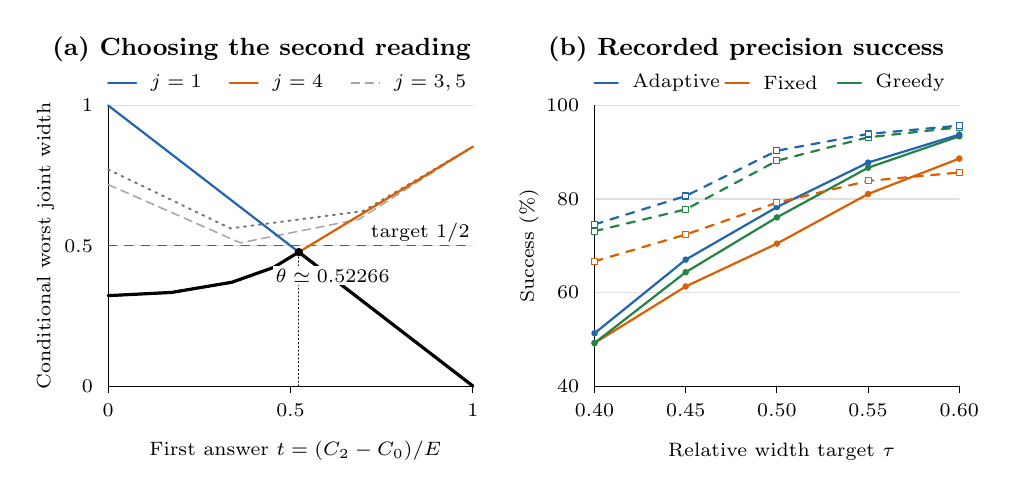
\begin{tikzpicture}[x=0.0098\linewidth,y=0.0098\linewidth,
font=\scriptsize,line cap=round,line join=round]
\definecolor{auditblue}{HTML}{2166AC}
\definecolor{auditorange}{HTML}{D95F02}
\definecolor{auditgreen}{HTML}{238443}
\node[anchor=west,font=\small\bfseries] at (0,47) {(a) Choosing the second reading};
\node[anchor=west,font=\small\bfseries] at (53,47) {(b) Recorded precision success};
\draw (7.000000,11) -- (7.000000,10.3);
\node[anchor=north] at (7.000000,10.1) {0};
\draw (26.500000,11) -- (26.500000,10.3);
\node[anchor=north] at (26.500000,10.1) {0.5};
\draw (46.000000,11) -- (46.000000,10.3);
\node[anchor=north] at (46.000000,10.1) {1};
\draw[black!12] (7,11.000000) -- (46,11.000000);
\node[anchor=east] at (6.4,11.000000) {0};
\draw[black!12] (7,26.000000) -- (46,26.000000);
\node[anchor=east] at (6.4,26.000000) {0.5};
\draw[black!12] (7,41.000000) -- (46,41.000000);
\node[anchor=east] at (6.4,41.000000) {1};
\draw (7,41) -- (7,11) -- (46,11);
\draw[dashed,black!65] (7,26) -- (46,26);
\node[anchor=south east,fill=white,inner sep=1pt] at (46,26) {target $1/2$};
\draw[black!35,densely dashed,line width=.55pt] (7.000000,32.542401) -- (21.137360,26.313235) -- (33.816702,28.829331) -- (46.000000,36.599285);
\draw[black!55,dotted,line width=.7pt] (7.000000,34.157622) -- (20.078835,27.853188) -- (34.270176,29.711230) -- (46.000000,36.599285);
\draw[auditblue,line width=.8pt] (7.000000,41.000000) -- (46.000000,11.000000);
\draw[auditorange,line width=.8pt] (7.000000,20.665739) -- (13.795865,21.011931) -- (20.236979,22.100812) -- (24.663467,23.672268) -- (46.000000,36.599285);
\draw[black,line width=1.15pt] (7.000000,20.665739) -- (13.795865,21.011931) -- (20.236979,22.100812) -- (24.663467,23.672268) -- (27.383609,25.320301) -- (46.000000,11.000000);
\draw[densely dotted] (27.383609,11) -- (27.383609,25.320301);
\fill (27.383609,25.320301) circle[radius=.45];
\node[anchor=north,fill=white,inner sep=1pt] at (31,23.9) {$\theta\simeq0.52266$};
\node[anchor=south] at (27,2) {First answer $t=(C_2-C_0)/E$};
\node[rotate=90] at (0.3,26) {Conditional worst joint width};
\draw[auditblue,line width=.8pt] (7,43.4) -- (10,43.4);
\node[anchor=west] at (10.5,43.4) {$j=1$};
\draw[auditorange,line width=.8pt] (20,43.4) -- (23,43.4);
\node[anchor=west] at (23.5,43.4) {$j=4$};
\draw[black!35,densely dashed] (33,43.4) -- (36,43.4);
\node[anchor=west] at (36.5,43.4) {$j=3,5$};
\draw[black!12] (59,11.000000) -- (98,11.000000);
\node[anchor=east] at (58.4,11.000000) {40};
\draw[black!12] (59,21.000000) -- (98,21.000000);
\node[anchor=east] at (58.4,21.000000) {60};
\draw[black!12] (59,31.000000) -- (98,31.000000);
\node[anchor=east] at (58.4,31.000000) {80};
\draw[black!12] (59,41.000000) -- (98,41.000000);
\node[anchor=east] at (58.4,41.000000) {100};
\draw (59.000000,11) -- (59.000000,10.3);
\node[anchor=north] at (59.000000,10.1) {0.40};
\draw (68.750000,11) -- (68.750000,10.3);
\node[anchor=north] at (68.750000,10.1) {0.45};
\draw (78.500000,11) -- (78.500000,10.3);
\node[anchor=north] at (78.500000,10.1) {0.50};
\draw (88.250000,11) -- (88.250000,10.3);
\node[anchor=north] at (88.250000,10.1) {0.55};
\draw (98.000000,11) -- (98.000000,10.3);
\node[anchor=north] at (98.000000,10.1) {0.60};
\draw (59,41) -- (59,11) -- (98,11);
\draw[auditorange,line width=.8pt] (59.000000,15.603175) -- (68.750000,21.647131) -- (78.500000,26.225885) -- (88.250000,31.537241) -- (98.000000,35.322344);
\fill[auditorange] (59.000000,15.603175) circle[radius=.35];
\fill[auditorange] (68.750000,21.647131) circle[radius=.35];
\fill[auditorange] (78.500000,26.225885) circle[radius=.35];
\fill[auditorange] (88.250000,31.537241) circle[radius=.35];
\fill[auditorange] (98.000000,35.322344) circle[radius=.35];
\draw[auditgreen,line width=.8pt] (59.000000,15.603175) -- (68.750000,23.173382) -- (78.500000,29.034188) -- (88.250000,34.345543) -- (98.000000,37.703297);
\fill[auditgreen] (59.000000,15.603175) circle[radius=.35];
\fill[auditgreen] (68.750000,23.173382) circle[radius=.35];
\fill[auditgreen] (78.500000,29.034188) circle[radius=.35];
\fill[auditgreen] (88.250000,34.345543) circle[radius=.35];
\fill[auditgreen] (98.000000,37.703297) circle[radius=.35];
\draw[auditblue,line width=.8pt] (59.000000,16.641026) -- (68.750000,24.516484) -- (78.500000,30.133089) -- (88.250000,34.894994) -- (98.000000,37.886447);
\fill[auditblue] (59.000000,16.641026) circle[radius=.35];
\fill[auditblue] (68.750000,24.516484) circle[radius=.35];
\fill[auditblue] (78.500000,30.133089) circle[radius=.35];
\fill[auditblue] (88.250000,34.894994) circle[radius=.35];
\fill[auditblue] (98.000000,37.886447) circle[radius=.35];
\draw[auditorange,line width=.8pt,dashed] (59.000000,24.333333) -- (68.750000,27.200717) -- (78.500000,30.605735) -- (88.250000,32.935484) -- (98.000000,33.831541);
\draw[auditorange,fill=white] (58.680000,24.013333) rectangle (59.320000,24.653333);
\draw[auditorange,fill=white] (68.430000,26.880717) rectangle (69.070000,27.520717);
\draw[auditorange,fill=white] (78.180000,30.285735) rectangle (78.820000,30.925735);
\draw[auditorange,fill=white] (87.930000,32.615484) rectangle (88.570000,33.255484);
\draw[auditorange,fill=white] (97.680000,33.511541) rectangle (98.320000,34.151541);
\draw[auditgreen,line width=.8pt,dashed] (59.000000,27.559140) -- (68.750000,29.888889) -- (78.500000,35.086022) -- (88.250000,37.594982) -- (98.000000,38.670251);
\draw[auditgreen,fill=white] (58.680000,27.239140) rectangle (59.320000,27.879140);
\draw[auditgreen,fill=white] (68.430000,29.568889) rectangle (69.070000,30.208889);
\draw[auditgreen,fill=white] (78.180000,34.766022) rectangle (78.820000,35.406022);
\draw[auditgreen,fill=white] (87.930000,37.274982) rectangle (88.570000,37.914982);
\draw[auditgreen,fill=white] (97.680000,38.350251) rectangle (98.320000,38.990251);
\draw[auditblue,line width=.8pt,dashed] (59.000000,28.275986) -- (68.750000,31.322581) -- (78.500000,36.161290) -- (88.250000,37.953405) -- (98.000000,38.849462);
\draw[auditblue,fill=white] (58.680000,27.955986) rectangle (59.320000,28.595986);
\draw[auditblue,fill=white] (68.430000,31.002581) rectangle (69.070000,31.642581);
\draw[auditblue,fill=white] (78.180000,35.841290) rectangle (78.820000,36.481290);
\draw[auditblue,fill=white] (87.930000,37.633405) rectangle (88.570000,38.273405);
\draw[auditblue,fill=white] (97.680000,38.529462) rectangle (98.320000,39.169462);
\node[anchor=south] at (79,2) {Relative width target $\tau$};
\node[rotate=90] at (52,26) {Success (\%)};
\draw[auditblue,line width=.8pt] (59,43.4) -- (61.5,43.4);
\node[anchor=west] at (62,43.4) {Adaptive};
\draw[auditorange,line width=.8pt] (73,43.4) -- (75.5,43.4);
\node[anchor=west] at (76,43.4) {Fixed};
\draw[auditgreen,line width=.8pt] (85,43.4) -- (87.5,43.4);
\node[anchor=west] at (88,43.4) {Greedy};
\end{tikzpicture}
\caption{An acquisition rule and its recorded outcomes. (a) Exact conditional envelopes from the saved HPM~1 comparison on 5 July 2025, 12:00--18:00 UTC, after querying boundary~2. Gray curves show the other second-query options; the black lower envelope selects boundary~4 below the switch and boundary~1 above it. Its maximum is about $0.47734$, below the half-width target for every possible first answer. (b) The adaptive, fixed-batch and greedy policies on all 819 original and 279 external blocks at five reporting targets. Solid curves represent the original panel and dashed curves the external panel. These exploratory recorded success rates use the existing $10^{-8}$ comparison tolerance; they are not worst-case precision probabilities.}
\label{fig:practical-guarantee-replay}
\end{figure}
